\chapter{Fundamenta\c c\~ao Te\'orica}
No cap\'itulo anterior foram abordadas algumas das pesquisas sobre o tema. Neste cap\'itulo ser\'a definido o
problema de planejamento energ\'etico para o caso hidrot\'ermico e a estrutura do planejamento baseado na Programa\c c\~ao
Din\^amica Dual Estoc\'astica.
\section{Despacho de energia}
No gerenciamento e transmiss\~ao da energia el\'etrica, o Brasil possui o Sistema Interligado Nacional
(SIN)\abbrev{SIN}{Sistema Interligado Nacional}
gerenciado pelo Operador Nacional de Energia (ONS)\abbrev{ONS}{Operador Nacional de Energia}
 correspondendo as regi\~oes Sul, Sudeste, Centro-Oeste, Nordeste e parte do Norte. O SIN \'e respons\'avel por abrigar cerca de
$96,6\%$ de toda a capacidade de produ\c c\~ao de energia do Brasil, seja por meio de fontes internas de energia
ou pela importa\c c\~ao de energia como ocorre na usina de Itaipu mediante o controle compartilhado com o
Paraguai\cite{an}. A ado\c c\~ao do SIN \'e justificada tendo por base: o interc\^ambio energ\'etico, a
complementaridade entre fontes de gera\c c\~ao de energia e pela sua capacidade de expans\~ao.

O interc\^ambio energ\'etico permite que regi\~oes que estejam vinculada ao SIN possam auxiliar no suprimento da
demanda de outras de regi\~oes que por algum fator interno ou externo n\~ao conseguem manter a demanda na sua localidade\cite{an}. Por
exemplo, considerando-se que determinadas regi\~oes brasileiras podem sofrer com a escassez de chuva o que implica na
baixa pluviosidade. Essa regi\~ao corre o risco de enfrentar problemas de abastecimento caso sua fonte de gera\c c\~ao
de energia el\'etrica seja por meio de hidrel\'etricas. Nesse tipo de situa\c c\~ao \'e totalmente poss\'ivel que outra
regi\~ao que n\~ao esteja enfrentando problemas de escassez, auxiliar enviando energia el\'etrica para atender a
localidade que esteja enfretando problemas de abastecimento. 

A complementaridade entre fontes de energia tem o mesmo princ\'ipio do interc\^ambio, contudo seu principal objetivo \'e permitir
que uma ou mais regi\~oes sejam abastecidas por diferente tipos de fonte de energia no intuito do sistema funcionar
da melhor forma poss\'ivel \cite{tom}. Isto \'e, localizadades que possuem como sua principal fonte de energia a
hidrel\'etrica podem sofrer com o baixos \'indices de seus reservat\'orios. Nesse tipo de situa\c c\~ao
\'e comum a ativa\c c\~ao de termel\'etricas para auxiliar o abastecimento. Esse \'e um exemplo t\'ipico de
complementaridade oferecido pelo SIN. 

Uma vez que a energia el\'etrica gerada pela hidrel\'etrica possui um custo menor
que a mesma quantidade de energia el\'etrica produzida por uma termel\'etrica, portanto, deve-se manter como meta a utiliza\c c\~ao
da hidrel\'etrica para diminui poss\'iveis custos ao consumido\cite{tom}. Contudo, apesar da termel\'etrica possui um
custo maior para a gera\c c\~ao de energia essa n\~ao possui o problema de abastecimento da hidrel\'etrica.
Portanto, a complementaridade para este caso seria configurar a utiliza\c c\~ao da hidrel\'etrica para a maioria dos
casos e a ativa\c c\~ao da termel\'etrica para auxiliar caso houvesse um pico de demanda ou problemas de
abastecimento por fatores como a pluviosidade.  

A expans\~ao \'e caracterizada por permitir que o SIN ao longo do tempo tenha condi\c c\~oes de assimilar outras hidrel\'etricas ou
regi\~oes permitindo que o sistema possua condi\c c\~oes de garantir a demanda mesmo com o aumento do consumo ou
poss\'iveis problemas de abastecimento por outros fatores internos ou externos. Por exemplo, em 2003 o SIN possuia 77,6
mil quil\^ometros de rede no per\'iodo de 2008 sua extens\~ao era 89,2 mil quil\^ometros de rede \cite{an}. 

O custo associado a produ\c c\~ao de energia \'e uma das vari\'aveis que influ\^encia o pre\c co. Na an\'alise do
sistema o pre\c co varia conforme o tipo de energia utilizada \cite{an}. Desta forma, o planejamento energ\'etico
depende do custo de produ\c c\~ao para determinar o despacho de energia. O despacho de energia \'e definido como quais
usinas devem ser mantidas ativas e quais precisam ser desativadas tomando-se em considera\c c\~ao a demanda, a oferta e
o custo de produ\c c\~ao do sistema.

Na an\'alise do custo de produ\c c\~ao para o despacho de energia outro fator a ser considerado s\~ao os sistemas
isolados. Os sistemas isolados est\~ao localizados principalmente na regi\~ao Norte,
estados como Amazonas, Roraima, Acre, Amap\'a e Rond\^onia. Esta denomina\c c\~ao deve-se por n\~ao estarem interligados ao
SIN e por n\~ao permitirem um interc\^ambio com outras regi\~oes devido as caracter\'istricas geogr\'aficas. O
funcionamento dos sistemas isolados \'e predominantemente t\'ermico. Os custos para a gera\c c\~ao de energia nesses sistemas s\~ao
superiores ao SIN por serem predominantemente t\'ermicos e pela sua localiza\c c\~ao requerer alto custo no
transporte de combust\'iveis \cite{an}. Como alternativa para o barateamento da energia gerada pelos sistemas isolados
foi constitu\'ido imposto denominado Conta de Consumo de Combust\'iveis (CCC)\abbrev{CCC}{Conta de Consumo de
Combust\'iveis}
que permite subs\'idiar a compra de
combust\'ivies garantindo que popula\c c\~ao dessas localidades tenha alguns dos benef\'icios do SIN. 

A produ\c c\~ao de eletricidade no sistema brasileiro tem como objetivo principal minimizar
os custo de opera\c c\~ao e garantir o suprimento de energia em todo o pa\'is \cite{tom}. Devido ao SIN ser
constitu\'ido predominantemente por um sistema hidrot\'ermico(hidrel\'etricas e termel\'etricas em regime de
complementaridade) este \'e afetado pela incerteza associada a pluviosidade
das regi\~oes que o constituem\cite{an}. Al\'em da pluviosidade o sistema hidrot\'ermico brasileiro \'e constitu\'ido
pelas seguinte caracter\'isticas:
\begin{itemize}
	\item \textit{Sazonalidade intra natural}. Al\'em da variabilidade natural ocorre um varia\c c\~ao entre as esta\c
		c\~oes do ano. 
	\item \textit{A complementariedade e diversidade regional}. As bacias brasileiras possuem caracter\'isticas
		f\'isicas e clim\'aticas distintas. Outro ponto a ser observado \'e que no momento que ocorre um estiagem no
		Nordeste as bacias do Sul podem est\'a com um alto n\'ivel dos reservat\'orios dada a pluviosidade da regi\~ao,
		ou seja, h\'a uma complementariedade entre as regi\~oes do Brasil.
	\item \textit{O acoplamento espacial}. Na estrutura de cascata as usinas que est\~ao mais perto da jusante possuem depend\^encia
		de usinas mais perto da montante.
	\item \textit{O acoplamento temporal}. Na estrutura de cascata decis\~oes sobre a utiliza\c c\~ao possuem
		consequ\^encias no futuro. 
	\item \textit{Custo term\'eletrico}. Usinas term\'eletricas possuem um custo alto de produ\c c\~ao el\'etrica em
		rela\c c\~ao as hidrel\'etricas.
	\item \textit{Aspecto ambiental}. Usinas termel\'etricas possuem um alto impacto ambiental ocasionado pela queima de
		combust\'ivel.
\end{itemize}

As caracterist\'icas mencionadas caracterizam o problema de despacho de energia hidrot\'ermico. A \fig{st}  exemplificar
o acoplamento temporal e espacial entre as usinas em cascata.
\begin{figure}[!htpb]
  \centering
  \resizebox{0.6\textwidth}{!}{%
  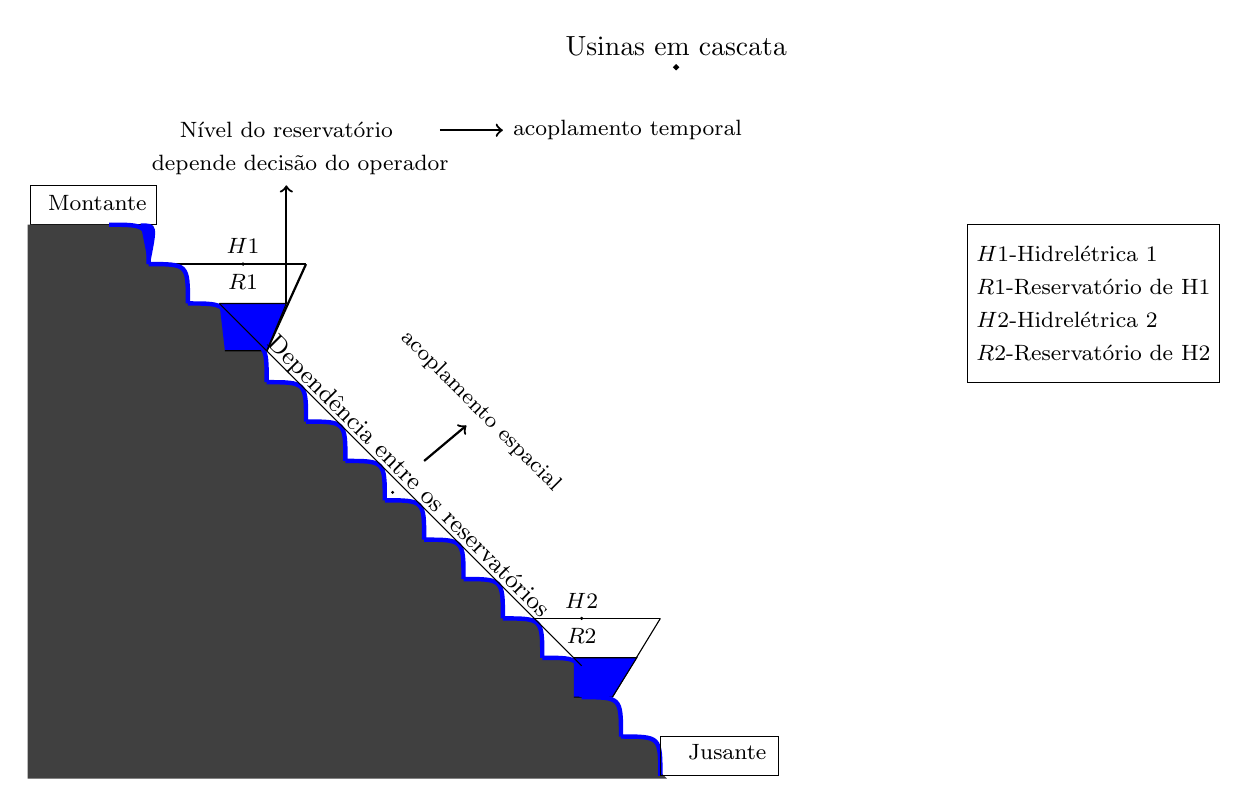
\begin{tikzpicture}
  % Desenho da cascata
  \draw [ultra thick,black] (7.2,9.0) circle (0.01mm) node[above]{Usinas em cascata};
  %
  % Desenho da montante
  \draw (-1.0,7.0) rectangle (0.6, 7.5) 
  node[below left] {\footnotesize Montante};
  %
  % Desenho da jusante

  \draw [thick, black]  (-1,0)--(-1,7);
  \draw [thick, black]  (-1,0)--(7,0);
  \draw [fill=darkgray] (-1.0,7.0) .. controls (0.5,7.0) .. (0.5,6.5);
  \draw [fill=darkgray] (0.0,7.0) .. controls (0.5,7.0) .. (0.5,6.5);
  \draw [fill=darkgray] (0.5,6.5) .. controls (1.0,6.5) .. (1.0,6.0);
  \draw [fill=darkgray] (1.0,6.0) .. controls (1.5,6.0) .. (1.5,5.5);
  \draw [fill=darkgray] (1.5,5.5) .. controls (2.0,5.5) .. (2.0,5.0);
  \draw [fill=darkgray] (2.0,5.0) .. controls (2.5,5.0) .. (2.5,4.5);
  \draw [fill=darkgray] (2.5,4.5) .. controls (3.0,4.5) .. (3.0,4.0);
  \draw [fill=darkgray] (3.0,4.0) .. controls (3.5,4.0) .. (3.5,3.5);
  \draw [fill=darkgray] (3.5,3.5) .. controls (4.0,3.5) .. (4.0,3.0);
  \draw [fill=darkgray] (4.0,3.0) .. controls (4.5,3.0) .. (4.5,2.5);
  \draw [fill=darkgray] (4.5,2.5) .. controls (5.0,2.5) .. (5.0,2.0);
  \draw [fill=darkgray] (5.0,2.0) .. controls (5.5,2.0) .. (5.5,1.5);
  \draw [fill=darkgray] (5.5,1.5) .. controls (6.0,1.5) .. (6.0,1.0);
  \draw [fill=darkgray] (6.0,1.0) .. controls (6.5,1.0) .. (6.5,0.5);
  \draw [fill=darkgray] (6.5,0.5) .. controls (7.0,0.5) .. (7.0,0.0);
  \draw [fill=darkgray,line width=0.1pt, opacity=100] (0,7)--(7,0);
  \filldraw [darkgray, line width=2.0pt] (0,7)--(7,0)--(-1,0)--(-1,7);
  %
  % Desenho de H1 
  \draw [thick, black] (1.7,6.5) circle (0.01mm) node [above]{\footnotesize $H1$};
  \draw [thick, black] (0.5,6.5)--(2.5,6.5);
  \draw [thick, black] (1.7,6.5) circle (0.01mm) node [below]{\footnotesize $R1$};
  \draw [thick, black] (2.5,6.5)--(2.0,5.4);
  
  \draw [fill=blue](1.40,6.0)--(2.25,6.0)--(2.0,5.4)--(1.47,5.4);
  % 
  % Desenho de H2
  \draw [thick, black] (6.0, 2.0) circle (0.01mm) node[above]{ \footnotesize $H2$};
  \draw [fill=darkgray] (5.0,2.0) -- (7.0,2.0);
  \draw [thick, black] (6.0,2.0) circle (0.01mm) node [below]{\footnotesize $R2$};
  \draw [fill=darkgray] (7.0,2.0) -- (6.39,1.0);
  \draw [fill=blue] (5.9,1.5) -- (6.7,1.5) --(6.39,1.0) -- (5.9, 1.0); 
  %
  % Desenho fio de agua
  \filldraw [blue, line width=1pt] (0.4, 7.0) .. controls (0.6, 7.0) .. (0.5,6.5);

  \draw [blue, ultra thick] (0.0,7.0) .. controls (0.5,7.0) .. (0.5,6.5);
  \draw [blue, ultra thick] (0.5,6.5) .. controls (1.0,6.5) .. (1.0,6.0);
  \draw [blue, ultra thick] (1.0,6.0) .. controls (1.5,6.0) .. (1.5,5.5);
  \draw [blue, ultra thick] (1.5,5.5) .. controls (2.0,5.5) .. (2.0,5.0);
  \draw [blue, ultra thick] (2.0,5.0) .. controls (2.5,5.0) .. (2.5,4.5);
  \draw [blue, ultra thick] (2.5,4.5) .. controls (3.0,4.5) .. (3.0,4.0);
  \draw [blue, ultra thick] (3.0,4.0) .. controls (3.5,4.0) .. (3.5,3.5);
  \draw [blue, ultra thick] (3.5,3.5) .. controls (4.0,3.5) .. (4.0,3.0);
  \draw [blue, ultra thick] (4.0,3.0) .. controls (4.5,3.0) .. (4.5,2.5);
  \draw [blue, ultra thick] (4.5,2.5) .. controls (5.0,2.5) .. (5.0,2.0);
  \draw [blue, ultra thick] (5.0,2.0) .. controls (5.5,2.0) .. (5.5,1.5);
  \draw [blue, ultra thick] (5.5,1.5) .. controls (6.0,1.5) .. (6.0,1.0);
  \draw [blue, ultra thick] (6.0,1.0) .. controls (6.5,1.0) .. (6.5,0.5);
  \draw [blue, ultra thick] (6.5,0.5) .. controls (7.0,0.5) .. (7.0,0.0);
  %
  % Desenho da legenda
   \node [draw,align=justify, minimum size=2cm]() at (12.5,6.0) {\footnotesize $H1$-\footnotesize Hidrel\'etrica 1 \\
  \footnotesize $R1$-\footnotesize Reservat\'orio de H1 \\ 
  \footnotesize $H2$-\footnotesize Hidrel\'etrica 2 \\
  \footnotesize $R2$-\footnotesize Reservat\'orio de H2};
  %\draw (9.5,4.5) rectangle (13.5,7.0); 
  %\draw (11.0,6.5) circle (0.01mm) node[] {\footnotesize $H1$-\footnotesize Hidrel\'etrica 1};
  %\draw (11.3,6.0) circle (0.01mm) node[] {\footnotesize $R1$-\footnotesize Reservat\'orio de H1};
  %\draw (11.0,5.5) circle (0.01mm) node[] {\footnotesize $H2$-\footnotesize Hidrel\'etrica 2};
  %\draw (11.3,5.0) circle (0.01mm) node[] {\footnotesize $R2$-\footnotesize Reservat\'orio de H2};
  %
  % Desenho do acoplamento temporal
  \draw (1.4,6)--(6,1.4);
  \draw [thick, black] (3.6,3.6) circle (0.01mm) node[above, rotate=315]{\fontsize{9}{12}\selectfont {Depend\^encia entre os
  reservat\'orios}};
  \draw [->,thick, black,rotate around={-50:(4.0,4.0)}]
	(4.0,4.0)--(4.0,4.7)node[above, rotate=315]{\footnotesize acoplamento espacial};
	\draw [->,thick, black](2.25,6.0)--(2.25,7.5) node[above,align=center]{\footnotesize N\'ivel do reservat\'orio 
	\\ \quad \footnotesize depende decis\~ao do operador};
	\draw [->,thick, black] (4.2,8.2) -- (5.0,8.2) node[right] {\footnotesize acoplamento temporal};
	%
	% Desenho da Jusante
	\draw (7.0,0.0) rectangle (8.5, 0.5);
	\draw (7.8,0.3) circle (0.01mm) node[]{\footnotesize{} Jusante};  
\end{tikzpicture}
}
  \caption{Representa\c c\~ao do acoplamento espacial e temporal.}
  \label{st}
\end{figure}

Portanto, no planejamento do despacho hidrot\'ermico a demanda do sistema deve ser garantida de forma a n\~ao prejudicar o
abastecimento, ao mesmo tempo a gera\c c\~ao term\'eletrica associada aos sistemas isolados possui um custo elevado. 
Esse custo deve ser considerado para n\~ao ocasionar um
aumento desagrad\'avel no pre\c co  associado ao sistema de energia brasileiro. 
Nesse contexto, um defini\c c\~ao mais ampla de despacho de energia seria o planejamento 
eficiente do sistema energ\'etico observando caracter\'isticas como, demanda, oferta, custo e
  as configura\c c\~oes do sistema. Para sistemas
 hidrot\'ermicos as caracter\'isticas do despacho podem ser resumidas no dilema do
 ``operador'' dado pelo diagrama a seguir.
 \begin{figure}[!h]
 \centering
 \resizebox{0.8\textwidth}{!}{%
  \xymatrix@=1.0em{
	& & *+[F]{\text{CHUVA}} \ar[r]& *+[F]{\text{DECIS\~AO CORRETA}}\\
	& *+[F]{\text {USAR \ RESERVAT\'ORIO}} \ar[ur] \ar[dr] & &\\
	& & *+[F]{\text{SECA}} \ar[r] & *+[F]{\text{PREJU\'IZO}} \\
	*+ [F]{\text {OPERADOR}} \ar[uur] \ar[ddr] & & & \\
	& & *+[F]{ \text {CHUVA}} \ar[r] & *+ [F]{\text{PREJU\'IZO}}\\
	& *+ [F]{\text {USAR TERMEL\'ETRICA}} \ar[ur] \ar[dr]& &\\
	& & *+[F] {\text {SECA}} \ar[r] & *+[F]{\text{DECIS\~AO CORRETA}}
 }}
 \caption {Dilema do operador.}  
 \label{dilop}
 \end{figure}

 Conforme o diagrama na \fig{dilop} o operador do sistema pode ter preju\'izo associado a sua escolha dado o componente
 estoc\'astico
relacionado aos
reservat\'orios das hidrel\'etricas. Pela complexidade do sistema hidrot\'ermico
brasileiro este tipo de decis\~ao possui um grau de dificuldade que transcede a simplicidade. Portanto, o sistema
hidrot\'ermico brasileiro possui caracter\'isticas que dificultam o planejamento por esse ser sucet\'ivel a mudan\c cas
ambientais e picos de demanda. Uma vez que o problema de despacho de energia para o caso hidrot\'ermico foi definido 
a pr\'oxima se\c c\~ao estabelece o modelo de programa\c c\~ao din\^amica dual estoc\'astica utilizado no planejamento
energ\'etico para o caso hidrot\'ermico. 
\section{Programa\c c\~ao Din\^amica Dual Estoc\'astica}
Na constru\c c\~ao do modelo considera-se primeiramente o caso determin\'istico supondo um problema de opera\c
c\~ao em dois est\'agios de tal forma que 
aflu\^encia em cada usina hidrel\'etrica em qualquer est\'agio do tempo \'e conhecida \cite{cp}. Desta forma,
podendo-se modelar o problema por:\symbl{$c_i,x_i$}{Vetores do $R^n$ com $i = 1, 2 , \dots$}
\symbl{$\geq$}{Maior ou igual que}
\symbl{$ \min $}{Minimiza\c c\~ao}
\pagebreak
\begin{align}
\label{t1}
&\min \langle c_1,x_1\rangle + \langle c_2,x_2\rangle \nonumber \\
&\mbox{tal que: }	A_1 x_1 \geq b_1 \\
&E_1 x_1 + A_2 x_2 \geq b_2 \nonumber
\end{align}
\begin{itemize}
  \item $c_1$ e $c_2$ s\~ao vetores que representam os custos relacionados ao 1 e 2 est\'agio respectivamente;
  \item $x_1$ e $x_2$ s\~ao vetores que representam as decis\~oes tomadas 1 e 2 est\'agios respectivamente;
  \item $b_1$ e $b_2$  s\~ao os vetores de recursos no 1 e 2 est\'agios respectivamente;
  \item $A_1$ e $A_2$ s\~ao matrizes que representam o acoplamento espacial;
  \item $E_1$ \'e uma matriz que descreve o acoplamento temporal.
\end{itemize}

\symbl{$\langle c_1,x_1\rangle$}{Produto Interno Euclidiano}
\symbl{$A_i, B_i, E_i$}{Matrizes de dimens\~ao $(m,n)$, para $i = 1,2, \dots$}
Observando-se o modelo \ref{t1} nota-se que a fun\c c\~ao a ser minizada \'e o custo em cada est\'agio do sistema. O
per\'iodo de tempo do est\'agio a ser analizado
depende do operador do sistema podendo ser dado por dia, semana, m\^es e ano. O tempo
utilizado para o planejamento do sistema possui uma relev\^ancia consider\'avel. Uma vez que o planejamento para um
per\'iodo de tempo suficiente longo ocorre a perca de informa\c c\~oes advindas das mudan\c cas naturais ou artificiais
que ocorrem no ambiente \cite{tom}. As usinas em cascata possuem o acoplamento  temporal e o
acoplamento espacial. Portanto, para a viabilidade do planejamento tais caracter\'istica devem ser consideradas no
modelo \ref{t1}. Dessa forma, as matrizes $A_1, A_2$  e $E_1$ caracterizam o comportamento natural das usinas no planejamento.
O problema descrito no modelo \ref{t1} pode ser interpretado como uma decis\~ao em dois est\'agios. O problema de dois
est\'agios \'e representado pelo
diagrama na \fig{estagio}.
\begin{figure}[!h]
 \centering
 \resizebox{0.8\textwidth}{!}{%
  \xymatrix@=1.0em{
	  & & *+[F]{\text{PLANEJAMENTO}}\ar[d]&\\ 
	  & & *+[F]{\text{CONFIGURA\c C\~AO INICIAL}} \ar[d]&\\  
	  & & *+[F]{\text{1 EST\'AGIO}} \ar[r] \ar[d]& *+[F]{\text{DECIS\~AO VI\'AVEL}} \ar[dd]\\
	  & & *+[F]{\text{CUSTO}} &\\   
	  & & & *+[F]{\text{2 EST\'AGIO}} \ar[d] \\ 
	  & & & *+[F]{\text{CUSTO}} 
}}
\caption{Representa\c c\~ao dos est\'agios.}
 \label{estagio}
\end{figure}
\symbl{$D$}{Conjunto vi\'avel pertecendo ao $R^n$}
\symbl{$f(x)$}{Fun\c c\~ao objetivo }
\symbl{$\Psi$}{Subconjunto do $R^n$}
\symbl{$R^n$}{Espa\c co Euclidiano}

O problema abordado pelo modelo \ref{t1}  \'e um problema de programa\c c\~ao linear \cite{alexey}. Portanto, para
a resolu\c c\~ao e interpreta\c c\~ao correta do modelo \'e necess\'ario os principais conceitos de otimiza\c c\~ao. O problema de otimiza\c c\~ao \'e definido por: dados dois conjuntos 
  $D $ e $\Psi$ subconjuntos do $\mathbb {R}^n$ e uma  fun\c c\~ao $f: \Psi
  \rightarrow R$ o objetivo \'e encontrar um minimizador de $f$ no conjunto $D$ \cite{alexey}. Isto \'e, 
  	\begin{align}%DEFINITION  OF FUNCTION OBJECTIVE 
		\label {obj}
	  	\min_{x\in D} f(x), 
	\end{align}
  define-se o conjunto D como o conjunto vi\'avel do problema, os pontos de D ser\~ao chamados pontos vi\'aveis e $f$ ser\'a chamada
  de fun\c c\~ao objetivo. Nota-se que para modelo \ref{t1} tem-se que: 
  \begin{align}
	  f(x) = \langle c_1,x_1\rangle + \langle c_2,x_2\rangle.
	  \label{linear}
  \end{align}
  \symbl{$\in$}{Pertence}
  A fun\c c\~ao objetivo dada por \ref{linear} \'e linear. O conjunto vi\'avel $D$ \'e constitu\'ido por todos os pontos
  $x_1$ e $x_2$ que satisfazem as inequa\c c\~oes do modelo \ref{t1}, o conjunto vi\'avel possui fundamental
  import\^ancia para a caracteriza\c c\~ao adequada do problema representado no modelo \ref{t1}. Basicamente ser\'a
  considerado somente o caso do conjunto $D$ ser um conjunto poliedral em $R^n$, particularmente sendo convexo
  \cite{alexey}. Isto \'e, o conjunto $D$ pode ser definido pela intersec\c c\~ao de semi-espa\c cos e hiperplanos em $R^n$
  ou de forma equivalente,
  \symbl{$h_i, i = 1,2 \dots$}{Semi-espa\c co do $R^n$}
  \symbl{$\leq$}{Menor ou igual que}
  \symbl{$g_i, i \leq 1,2 \dots$}{Hiperplano do $R^n$}
  \begin{align}
  		D = \left \{ x \in \Psi; \begin{array}{cc} h_i(x) = 0, i = 1, \dots, l \\ g_j(x) \leq 0, j = 1, \dots, m
		\end{array} \right \}.
		\label{dpol}
  \end{align}
Portanto, as inequa\c c\~oes no modelo \ref{t1} representam os hiperplanos no $R^n$. A figura(\ref{poli}) ilustra a defini\c c\~ao \ref{dpol}.
	\begin{figure}[!h]%POLYHEDRAL SET
			\centering
			\resizebox{2.5\width}{!}{
			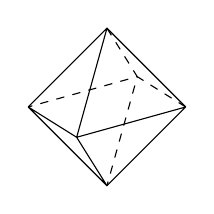
\begin{tikzpicture}
	\path
	( 1, 0, 0) coordinate (A1)
	( 0, 0,-1) coordinate (A2)
	(-1, 0, 0) coordinate (A3)
	( 0, 0, 1) coordinate (A4)
	( 0, 1, 0) coordinate (B1)
	( 0,-1, 0) coordinate (B2);

	\draw 
	(A1)--(A4)--(A3)
	(B1)--(A4)--(B2)
	(A1)--(B1)--(A3)
	(A1)--(B2)--(A3);

	\draw[dashed]
	(A1)--(A2)--(A3)
	(B1)--(A2)--(B2);
\end{tikzpicture}

			}
			\caption{Exemplo de um conjunto poliedral  $\mathbb{R}^3$.}
			\label{poli} 
		\end{figure}

  Finalmente para a caracteriza\c c\~ao completa do problema do modelo \ref{t1} a fun\c c\~ao objetivo $f(x)$ na qual se
  procura o ponto de m\'inimo pode apresentar restri\c c\~oes em seu dom\'inio por meio do conjunto vi\'avel $D$
  caracterizando os problemas com e sem restri\c c\~oes.  No problema descrito pelo modelo \ref{t1} o conjunto vi\'avel
  $D$ \'e caracterizado pelas inequa\c c\~oes ou hiperplanos, logo, um problema com restri\c c\~oes no dom\'inio da fun\c c\~ao
  objetivo \ref{linear}. Portanto, quando a fun\c c\~ao objetivo $f(x)$ do problema \ref{obj} \'e linear e o conjunto
  v\'iavel \'e poliedral, particularmente convexo essa caracteriza\c c\~ao recebe a denomina\c c\~ao de problema de
  programa\c c\~ao linear. A figura \ref{via} a seguir ilustrar as duas situa\c c\~oes para problemas do tipo \ref{obj}.

  \begin{figure}[!h]%THE VIABLE WITHOUT RESTRICTIONS 
		\centering
		\resizebox{0.7\width}{!}{
			  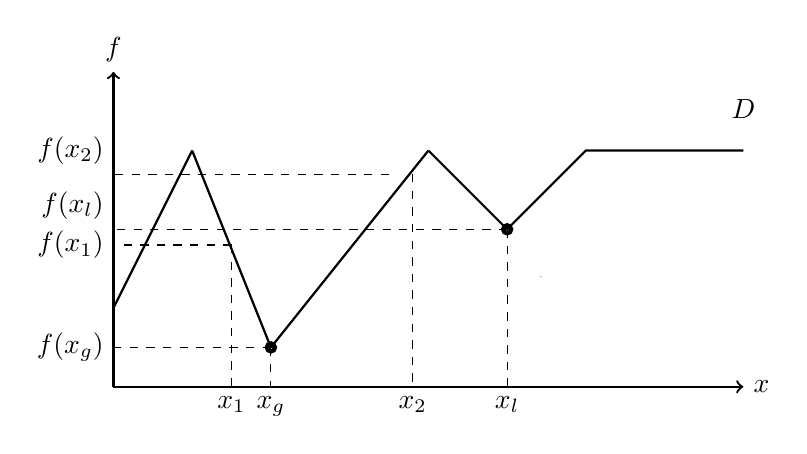
\begin{tikzpicture}
		\draw [->, thick, black] (0,0)--(8,0) node[right] {$x$};
		\draw [->, thick, black] (0,0)--(0,4) node[above] {$f$};
		\draw [thick, black] (0,1)--(1,3);
		\draw [thick, black] (1,3)--(2,0.5); 
		%\draw [thick, black] (1,3)--(2,0.5) node[above,xshift = 3,yshift = 16] {$G$};
		\draw [thick, black](2,0.5)--(4,3);
		\draw [thick, black](4,3)--(5,2); 
		%\draw [thick, black](4,3)--(5,2) node[below left] {$L$};
		\draw [thick, black](5,2)--(6,3)--(8,3)node[above,yshift=8] {$D$};
		%\draw [thick, black](5,2)--(6,3)--(8,3)node[above,yshift=8] {$D$};
		\draw [ultra thick, black](2,0.5) circle (0.5mm);
		\draw [ultra thick, black](5,2) circle (0.5mm);
		\draw [dashed, black](2,0.5)--(0,0.5) node[left] {$f(x_g)$} ;
		\draw [dashed, black](2,0.5)--(2,0) node[below] {$x_g$};
		\draw [dashed, black] (1.5,1.8)--(1.5,0) node[below] {$x_1$};
		\draw [dashed, black] (1.5,1.8)--(0.0,1.8) node[left] {$f(x_1)$};
		\draw [dashed, black](3.8,2.7)--(3.8,0) node[below] {$x_2$};
		\draw [dashed, black](3.5,2.7)--(0.0,2.7) node[above left] {$f(x_2)$};
		\draw [dashed, black](5,2)--(0,2) node[above left] {$f(x_l)$};
		\draw [dashed, black](5,2)--(5,0) node[below] {$x_l$};
		\draw [dashed, black](5,0)--(5,2);
	%	\draw [dashed, black](5,0)--(5,2) node[above, yshift = 8] {$U$};
		%\draw [thin, black] (5,2)--(5.7,1)[above left];
		\draw [very thin, black] (5.43,1.4) circle (0.01mm);  
		%\draw [very thin, black] (5.43,1.4) circle (0.01mm) node[above] {$\epsilon$};  
		%\draw [thin, black](5,2) circle (12.0mm); 
	  \end{tikzpicture}
 
  	}
	\resizebox{0.7\width}{!}{
		  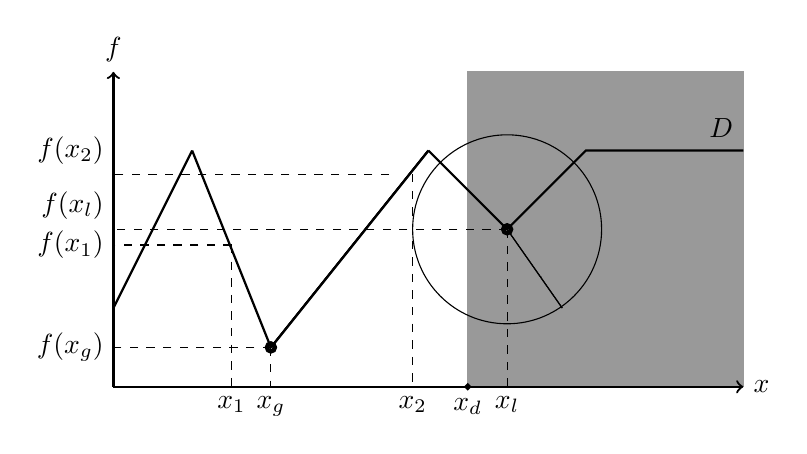
\begin{tikzpicture}
  \draw [->, thick, black] (0,0)--(8,0) node[right] {$x$};
  \draw [->, thick, black] (0,0)--(0,4) node[above] {$f$};
  \draw [thick, black] (0,1)--(1,3);
  \draw [thick, black] (1,3)--(2,0.5); 
  %\draw [thick, black] (1,3)--(2,0.5) node[above,xshift = 3,yshift = 16] {$G$};
  \draw [thick, black](2,0.5)--(4,3);
  \draw [thick, black](2,0.5)--(4,3);
  \draw [thick, black](4,3)--(5,2) ;
  %\draw [thick, black](4,3)--(5,2) node[below left] {$L$};
  \draw [thick, black](5,2)--(6,3)--(8,3)node[left,yshift=8] {$D$};
  \draw [ultra thick, black](2,0.5) circle (0.5mm);
  \draw [ultra thick, black](4.5,0) circle (0.1mm) node[below]{$x_d$};
  \draw [dashed, black](5,2)--(5,0) node[below] {$x_l$};
  \draw [ultra thick, black](5,2) circle (0.5mm);
  \fill [black, draw=black, opacity = 0.4] (4.5,0) rectangle (8,4);
  \draw [dashed, black](2,0.5)--(0,0.5) node[left] {$f(x_g)$};
  \draw [dashed, black](2,0.5)--(2,0) node[below] {$x_g$};
  \draw [dashed, black] (1.5,1.8)--(1.5,0) node[below] {$x_1$};
  \draw [dashed, black] (1.5,1.8)--(0.0,1.8) node[left] {$f(x_1)$};
  \draw [dashed, black](3.8,2.7)--(3.8,0) node[below] {$x_2$};
  \draw [dashed, black](3.5,2.7)--(0.0,2.7) node[above left] {$f(x_2)$};
  \draw [dashed, black](5,2)--(0,2) node[above left] {$f(x_l)$};
  \draw [very thin, black] (5.43,1.4) circle (0.01mm);  
  %\draw [very thin, black] (5.43,1.4) circle (0.01mm) node[above] {$\epsilon$};  
  \draw [thin, black] (5,2)--(5.7,1)[above left];
  \draw [dashed, black](5,0)--(5,2);
  %\draw [dashed, black](5,0)--(5,2) node[above, yshift = 8] {$U$};
  \draw [thin, black] (5,2)--(5.7,1)[above left];
  \draw [thin, black](5,2) circle (12.0mm); 
  \end{tikzpicture}
 
  	}
		\caption{Rela\c c\~ao entre o dom\'inio e o conjunto vi\'avel $D$.}
		\label{via}
  	\end{figure}

	A esquerda da figura \ref{via} representa o dom\'inio sem restri\c c\~oes, portanto o conjunto vi\'avel \'e todo o
	dom\'inio, por sua vez a direita da figura \ref{via} representa restri\c c\~oes ao dom\'inio, logo, o conjunto
	vi\'avel $D$ \'e um subconjunto do dom\'inio.  
O ponto de min\'imo de $f(x)$ que \'e a solu\c c\~ao do problema \ref{obj} \'e denominado ponto de \'otimo possuindo
como nomenclatura $x^{*}$. 
Para a  resolu\c c\~ao  do problema descrito em \ref{t1} \'e
escolhida uma decis\~ao vi\'avel $x_1$ para o 1 est\'agio sendo denotada por ${x_1}^{*}$ de tal forma que $A_1{x_1}^{*} \geq b_1$.
Nota-se que a priori n\~ao \'e poss\'ivel obter nenhuma informa\c c\~ao futura do sistema. Portanto, o operador do sistema
somente possui condi\c c\~oes para a escolha de uma configura\c c\~ao vi\'avel $x_1$, nesse caso supondo-se que a decis\~ao
\'e \'otima. 
Assim, o problema para decis\~ao do est\'agio 2 pode ser reescrito como, 
\begin{align}
  \begin{split}	
 & 	\min \langle c_2,x_2\rangle  \\
&\mbox{tal que: }A_2 x_2 \geq b_2 -{E_1 x_1}^{*}.
  \end{split}
    \label{p2}
\end{align}

O problema(\ref {p2}) \'e um problema de programa\c c\~ao linear e ${x_1}^{*}$ \'e conhecido (decis\~ao vi\'avel do
primeiro est\'agio)\cite{alexey}. 
Uma vez representadas
as decis\~oes vi\'aveis tomadas no est\'agio 1 do
problema o intuito \'e minimizar o custo da fun\c c\~ao objetivo para o 2 est\'agio. Dado que ${x_1}^{*}$ \'e vi\'avel procura-se uma solu\c c\~ao \'otima para $x_2$ representado por
${x_2}^{*}$. A solu\c c\~ao do est\'agio 2 depende das decis\~oes tomadas no est\'agio 1. Portanto, o
problema do est\'agio 2 pode ser visto como uma fun\c c\~ao do 1 est\'agio\cite{cp}, isto \'e,
\begin{align}
  \begin{split}	
	\alpha_{1} (x_1) =& \min \langle c_2,x_2\rangle \\
	&\mbox{tal que: }A_2 x_2 \geq b_2 - {E_1 x_1}^{*} 
  \end{split}
    \label{p3}
\end{align}
onde ${\alpha}_{1}$ representa o valor \'otimo para o est\'agio 2.
O problema \ref{t1} pode ser reescrito como se segue,
\begin{align}
  \begin{split}	
  &\min \langle c_1,x_1\rangle + {\alpha}_{1}(x_1) \\
&\mbox{tal que: }	A_1x_1 \geq b_1.
\end{split}
\label{linear2}
  \end{align}

No problema \ref{linear2} o conjunto vi\'avel possui uma depend\^encia tanto da decis\~ao vi\'avel do 1 est\'agio como
tamb\'em das decis\~oes do 2 est\'agio. Para o planejamento esse tipo de depend\^encia n\~ao \'e interessante, pois, o
ideal seria encontrar uma forma de minimizar o custo sem a depend\^encia das decis\~oes do 2 est\'agio. Nesse intuito pode-se
aplicar uma transforma\c c\~ao no problema \ref{linear2} para remover a depend\^encia das decis\~oes do 1 e 2 est\'agio
representadas pelo vetor $x_1$ e $x_2$. A t\'ecnica de transforma\c c\~ao \'e denominada dualidade \cite{boyd}, sendo definida a seguir.
\symbl{$R(m,n)$}{Espa\c co da matrizes (m,n)}
\symbl{$\max$}{Maximiza\c c\~ao}
\symbl{$\pi, \pi_i, i = 1, 2 \dots $}{Vari\'avel dual}
\symbl{$\alpha, \alpha_i, i = 1,2 \dots $}{Vari\'avel escalar}
	\begin{defin}%Dual of problem
		Considerando-se o seguinte problema de programa\c c\~ao de linear que ser\'a denominado de problema primal,
				\begin{align}
					\label {primal}
					\min \left < c,x \right >  \mbox{sujeito a} \hspace{2pt} x \in D = \{ x \in R^n;Bx \geq b \},
				\end{align}
				onde $b \in R^m$, $c \in R^n$ e $B \in R(m,n)$.\\

				O problema dual de \ref{primal} \'e definido como,
				\begin{align}
					\label {dual}
					\max \left<b,\mu \right> \mbox{sujeito a} \hspace{2pt} \mu \in \Delta = \{ \mu \in R_{+}^{m}; B^T\mu \leq c\}
				\end{align}
				onde $\mu$ \'e o vetor dual do problema.
				\label{du}
  	\end{defin}
	Aplicando-se a dualidade \ref{du} no problema (\ref{p2}) \'e imediato que,
\begin{align}
  \begin{split}	
 \alpha_{1}(x_1) = &\max \pi (b_2 - E_1x_1 ) \\
	&\mbox{tal que: }\pi A_2  \leq c_2.
  \end{split}
 	\label{p4}
\end{align}

Nas circunst\^ancias do problema a solu\c c\~ao da problema (\ref{p4}) \'e equivalente ao problema (\ref{p2}). De fato, 
assumindo-se que o problema (\ref{p2}) possui solu\c c\~ao, portando, o seu dual descrito por (\ref{p4}) admite o mesmo
conjuto de pontos \'otimos como solu\c c\~ao\cite{alexey}.
Nota-se que o conjunto vi\'avel $\pi A_2 \leq c_2$ do problema (\ref{p4}) n\~ao depende da decis\~ao $x_1$ e $x_2$. Desta forma, os
pontos extremos ou v\'ertices do conjunto vi\'avel podem ser caracterizados por $\pi = \left\{ \pi^1, \pi^2, \dots,
\pi^P \right\}$ \cite{cp}. Uma vez
que o problema de programa\c c\~ao linear descrito por (\ref{p4}) possua uma solu\c c\~ao. A sua solu\c c\~ao ser\'a  
um dos v\'ertice do conjunto vi\'avel\cite{alexey}.
Portanto, o problema descrito por (\ref{p4}) pode ser reescrito como se segue,
\begin{align*}
  \begin{aligned}
	{\alpha}_{1}(x_1) = \text {max} \ \ {\pi}^{i} (b_2 - E_1x_1) \\
	{\pi}^{i} \in  D_1 = \left\{ {\pi}^{1}, {\pi}^{2},\dots, {\pi}^{P} \right\}.
  \end{aligned}
\end{align*}

O conjunto $D_1$ representa o conjunto de v\'ertices do conjunto vi\'avel D.
Finalmente, o problema (\ref{p4}) pode ser reescrito para, 

\begin{align}
	\label{aux1}
  	\alpha_{1}(x_1) =& \min\alpha \nonumber \\ 
	&\mbox{tal que: }\alpha \geq \pi^{i}(b_2 - E_1 x_1) \\
	&\mbox{com } i = 1,2, \dots , P \nonumber
\end{align}
onde $\alpha$ \'e uma vari\'avel escalar. Por fim, fazendo-se a substitui\c c\~ao (\ref{aux1}) em (\ref{t1}) o problema
dado por \ref{t1} torna-se,
\begin{align}
	\label{fin1}
&\min \langle c_1,x_1\rangle + \alpha \nonumber\\
&\mbox{tal que: }	A_1 x_1 \geq b_1 \\
&	\pi^{i}(b_2 - E_1x_1) - \alpha \leq 0\nonumber \\ 
&\mbox{parar }	i = 1, 2, \dots , P.\nonumber
\end{align}

A t\'ecnica para problemas determin\'isticos utilizada para a formula\c c\~ao do problema \ref{fin1} \'e conhecida na literatura como
a decomposi\c c\~ao de Benders \cite{benders} ou cortes por hiperplanos. A ideia da t\'ecnica \'e decompor o problema original permitindo que esse
seja resolvido de forma iterativa por meio da resolu\c c\~ao de problemas auxiliares. Outro fator importante da
utiliza\c c\~ao da t\'ecnica de decomposi\c c\~ao de Benders \'e evidenciado na formula\c c\~ao dada em \ref{fin1}. Uma
vez que na formula\c c\~ao apresentada em \ref{fin1} nenhum do termos depende de $x_2$, ou seja, o planejamento pela
utiliza\c c\~ao da t\'ecnica de Benders independe das decis\~oes tomadas no 2 est\'agio. A import\^ancia desse fato
deve-se que o operador do sistema n\~ao necessita tomar decis\~aoes no 2 est\'agio para o planejamento o que diminuir a
complexidade do processo de planejamento e evitar poss\'iveis erros.
A descri\c c\~ao do algoritmo \'e
dada a seguir.

\begin{center}
Algoritmo do problema determin\'istico:\\
\end{center}
Resolve problema principal:
\begin{align*}
&\min \langle c_1,x_1\rangle + \alpha \nonumber\\
&\mbox{tal que: }	A_1 x_1 \geq b_1
\end{align*}
Na primeira verifica\c c\~ao simplesmente assumir valores vi\'aveis.\\
Chute inicial para o problema principal = $x_1^{*}$ e $\alpha$.\\
Repitar:\\
Resolver  o problema auxiliar (1):
\begin{align*}
  \begin{split}	
 \alpha_1 = &\max \pi (b_2 - E_1x_1 ) \\
	&\mbox{tal que: }\pi A_2  \leq c_2.
  \end{split}
\end{align*}

	Compara\c c\~ao de converg\^encia:
		\begin{align*}
			&|\alpha - \alpha_1|< \mbox{toler\^ancia}\\
			&\mbox{para;}\\
			&\mbox{Sair da repeti\c c\~ao;}\\
			&\mbox{Sa\'ida \'otima} = x_1^{*}, \alpha_1.
		\end{align*}

	Caso contr\'ario:\\

	Acrecente ao problema principal a condi\c c\~ao:
		\begin{align*}
			\pi(b_2 - E_1x_1) - \alpha \leq 0
		\end{align*}

	Resolver o problema principal:
		\begin{align*}
			&\min \langle c_1,x_1\rangle + \alpha \nonumber\\
			&\mbox{tal que: }	A_1 x_1 \geq b_1\\
			&\pi(b_2 - E_1x_1) - \alpha \leq 0
		\end{align*}
Voltar ao passo 1.\\
Atingido o número de itera\c c\~oes parar.\\
\symbl{$p(x)$}{Fun\c c\~ao de probabilidade}
\symbl{$E(x)$}{Valor Esperado}
A Programa\c c\~ao Din\^amica Dual Estoc\'astica consiste em uma aplica\c c\~ao da decomposi\c c\~ao de Benders em um problema cuja a
natureza \'e
estoc\'astica. Portanto, para o modelamento ser\'a apresentado a seguir os conceitos b\'asicos da teoria das
probabilidades 
utilizados na formula\c c\~ao do modelamento estoc\'astico.
Basicamente uma probabilidade deve garantir as seguintes propriedades,
	\begin{description}
		\centering
		\item $\rm{p_1}$: $ 0 \leq p(x_i) \leq 1, \forall i = 1,2, \dots $, 
		\item $\rm{p_2}$: $ \sum\limits_{i}^{} p(x_i)= 1. \qquad \qquad \quad \ \ \ \ $ 
  	\end{description} 

	Outro importante conceito utilizado no modelamento \'e o de valor esperado, esperan\c{c}a matem\'{a}tica, ou m\'{e}dia de
uma vari\'{a}vel aleat\'oria. A no\c c\~ao de valor esperado \'e extremamente \'{u}til na an\'{a}lise de fen\^{o}menos
aleat\'{o}rios justamente por
ser comportar como a m\'{e}dia permitindo informa\c{c}\~{o}es do problema observado.
Para o caso discreto \'e definido como, 
\symbl{$\sum$}{Somat\'orio}
	\begin{align}
		\label{dise}
		E(X) = \sum\limits_{i = 1}^{\infty}x_ip_X(x_i).
	\end{align}

Nota-se que o valor esperado \'e
definido como um somat\'orio na rela\c c\~ao \ref{dise}, pois, a vari\'avel aleat\'oria X \'e discreta, ou seja, assume
valores $x_i$ para $i= 1,2, \dots$\cite{magalhaes}. Por exemplo,
considerando-se o lan\c camento de um dado onde a vari\'avel X representar a face do dado. Desta forma, X \'e uma
vari\'avel discreta
e assume valores no conjunto
\symbl{$\omega_{ij},i = 1,2 \dots, j = 1,2 \dots  $}{Cen\'arios de probabilidade}
$\Omega = \{1,2,3,4,5,6\}$, onde $\Omega$ \'e o conjunto de todos os resultados poss\'iveis para o evento de
interesse \cite{james}.
Portanto, o valor esperado de X \'e dado por,
	\begin{align*}
		E(X) = \frac{1}{6}(1 + 2 + 3 + 4 + 5 + 6) = \frac{21}{6} = \frac{7}{2}
	\end{align*}
Nota-se que o valor de X nesse caso n\~ao pertence ao conjunto $\Omega$, isto \'e, o valor esperado indica qual o valor
que se espera para a repeti\c c\~ao do evento um n\'umero  $n$ vezes, sendo $n$ um n\'umero grande. Portanto, como todos
o resultados do evento descrito s\~ao equiprov\'aveis, logo, pode-se concluir que para a repeti\c c\~ao um n\'umero
suficiente grande de vezes a m\'edia aritm\'etica tende a $\frac{7}{2}$. Para o caso
cont\'{i}nuo, a ideia \'{e} an\'{a}loga,
	\begin{align*}
		E(X) = \int\limits_{-\infty}^{\infty} xf(x) dx.
	\end{align*}

Com conceitos de probabilidade estabelecidos. Seja o problema de dois est\'agios similar ao caso determin\'istico,
contudo o 2 est\'agio depende dos valores
que uma ou mais vari\'aveis aleat\'orias discretas podem assumir. Por exemplo, suponde-se que o vetor $b$ pode assumir dois
valores $b_1$ e $b_2$ com
probabilidades $p_1$ e $p_2$ respectivamente ($p_1 + p_2 = 1, p_i \geq 0$, $i = 1, 2$) \cite{cp}. O objetivo \'e encontrar a estrat\'egia que
minimiza o
valor do custo esperado. Portanto, o problema fica modelado por:
\begin{align}
	\label{aux2}
  z = \min  \langle c_1,x_1\rangle &+ p_1\langle c_2,x_{21}\rangle + p_2\langle c_2,x_{22}\rangle \nonumber\\	
 \mbox{tal que: }&	A_1 x_1 \geq b_1 \\
	&E_1 x_1 + A_2 x_{21} \geq b_{21} \nonumber\\
	&E_1 x_1 + A_2x_{22} \geq b_{22} \nonumber
\end{align}
O modelo descrito por \ref{aux2} possui considera\c c\~oes distintas do caso determin\'istico. Primeiramente, o termo
dado por $p_1\langle c_2,x_{21}\rangle + p_2\langle c_2,x_{22}\rangle $ \'e igual a $E(X_2)$, isto \'e, para a minimiza\c c\~ao da
fun\c c\~ao objetivo do modelo \ref{aux2} utiliza-se o valor esperado do custo no 2 est\'agio. Como o planejamento
considerar os dois cen\'arios de planejamento, portanto, para cada um dos cen\'arios deve-se considerar o acoplamento
temporal e o acoplamento espacial existente entre as usinas hidrel\'etricas no 2 est\'agio. Nota-se que a condi\c c\~ao
$A_1 x_1 \geq b_1$ permanece inalterada, pois, semelhantemente ao caso determin\'istico para o caso estoc\'astico o
1 est\'agio ainda depende somente da decis\~ao do operador do sistema dada as condi\c c\~oes do ambiente. 

O objetivo do
modelo no planejamento e encontrar o custo esperado. O custo esperado \'e calculado levando-se em considera\c c\~ao dois
custos parciais. Primeiramente \'e calculado o custo do primeiro est\'agio dada a escolha vi\'avel tomada pelo
operador do sistema. No segundo momento \'e calculado um custo parcial levando-se em consequ\^encia as decis\~oes do
operador do sistema tomadas no 1 est\'agio e as condi\c c\~oes ambientais como o volume dos reservat\'orios e quest\~oes 
relacionadas a demanda do sistema. A partir da obten\c c\~ao dos custos do 1 est\'agio e do 2 est\'agio \'e poss\'ivel
estipular o custo esperado para o planejamento do sistema no per\'iodo observado. 
O diagrama na Figura (\ref{estocastico}) a seguir representar o problema de planejamento de dois est\'agios para o caso
estoc\'astico de dois cen\'arios.

\begin{figure}[!h]
 \centering
 \resizebox{1.1\textwidth}{!}{%
  \xymatrix@=1.0em{
	  & & &*+[F]{\text{PLANEJAMENTO}}\ar[d]&\\ 
	  & & &*+[F]{\text{CONFIGURA\c C\~AO INICIAL}} \ar[d]&\\  
	  & & &*+[F]{\text{1 EST\'AGIO}} \ar[r] \ar[d]& *+[F]{\text{DECIS\~AO VI\'AVEL}} \ar[dd]\\
	  & & &*+[F]{\text{CUSTO}}& \\ 
	  & & && *+[F]{\text{2 EST\'AGIO}} \ar[dl] \ar[drrr]\\
	  & & & *+[F]{\text{CEN\'ARIO 1}} &
	  & & & *+[F]{\text{CEN\'ARIO 2}}\\
	  & & && *+[F]{\text{CUSTO ESPERADO NO 2 EST\'AGIO}}\ar[urrr] \ar[ul]
}}
\caption{Representa\c c\~ao dos est\'agios para o caso estoc\'astico.}
 \label{estocastico}
\end{figure}
Pelo diagrama na Figura (\ref{estocastico})e levando-se em considera\c c\~ao a decis\~ao vi\'avel $x_1^{*}$ tomada pelo
operador do sistema no 1 est\'agio o problema \ref {aux2} pode ser reescrito como,
{\setlength{\belowdisplayskip}{-10pt}
\begin{align*}
  z = \min  \langle c_1,x_1\rangle + p_1{\omega}_{21} + p_2 {\omega}_{22} \nonumber \\	
	A_1 x_1 \geq b_1
  \end{align*}%
\begin{align}
	\label{principal}
  \begin{split}	
  &\omega_{21}(x_1) =\min \langle c_2,x_{21}\rangle \\
  & A_2 x_{21} \geq b_{21} - E_1 x_1^{*} 
  \end{split}
	\end{align}}%
\begin{align}
  \begin{split}	
 	&\omega_{22}(x_1) = \min  \langle c_2,x_{22}\rangle \\ \nonumber
	&A_2x_{22} \geq b_{22} - E_1 x_1^{*}. 
  \end{split}
   \end{align}%

A formula\c c\~ao do problema dado em \ref{principal} decomp\~oe o problema principal em um problema derivado com dois
subproblemas auxiliares. O problema principal derivado \'e dado por,

{\setlength{\abovedisplayskip}{-15pt}
\begin{align}
	\label{estoPrincipal}
  z = \min  \langle c_1,x_1\rangle + p_1{\omega}_{21} + p_2 {\omega}_{22} \nonumber \\	
	A_1 x_1 \geq b_1.
\end{align}}

Os problemas auxiliares s\~ao:
{\setlength{\belowdisplayskip}{-5pt}
\begin{align}
	\label{estoAux1}
  \begin{split}	
  	&\omega_{21}(x_1) =\min \langle c_2,x_{21}\rangle \\
  	& A_2 x_{21} \geq b_{21} - E_1 x_1^{*} 
  \end{split}
\end{align}}
\begin{align}
	\label{estoAux2}
	\begin{split}	
 		&\omega_{22}(x_1) = \min  \langle c_2,x_{22}\rangle \\
		&A_2x_{22} \geq b_{22} - E_1 x_1^{*}. 
	\end{split}
\end{align}
Os subproblemas \ref{estoAux1} e \ref{estoAux2} representam os cen\'arios 1 e 2 considerados no planejamento respectivamente.
Nota-se que os problemas  \ref{estoPrincipal}, \ref{estoAux1} e \ref{estoAux2} s\~ao todos problemas de programa\c c\~ao
linear. De modo an\'aloga ao caso determ\'inistico aplica-se a dualidade nos problemas \ref{estoAux1} e \ref{estoAux2}
obtendo-se:
\begin{align}
  \begin{split}	
	  \omega_{21}(x_1) = &\max \pi_1 (b_{21} - E_1x_1 ) \\
	&\mbox{tal que: }\pi_1 A_2  \leq c_2.
  \end{split}
 	\label{auxdual1}
\end{align}
\begin{align}
  \begin{split}	
	  \omega_{22}(x_1) = &\max \pi_2 (b_{22} - E_1x_1 ) \\
	&\mbox{tal que: }\pi_2 A_2  \leq c_2.
  \end{split}
 	\label{auxdual2}
\end{align}
Em seguida, aplicando a decomposi\c c\~ao de Benders nos problemas \ref{auxdual1} e \ref{auxdual2} obt\^em-se:  
\symbl{$\beta_i, i = 1, 2 \dots$}{Vari\'avel escalar}
\begin{align}
	\label{auxb1}
&\omega_{21}(x_1) = \min  \beta_{1}\nonumber \\
	&\mbox{tal que: }\beta_{1}  \geq {\pi}_{1}^{i}b_{21} - E_1 x_1 \\
	&\mbox{para }i = 1,2,\dots, P  \nonumber
  \end{align}
\begin{align}
	\label{auxb2}
&\omega_{22}(x_1) = \min  \beta_{2}\nonumber \\
	&\mbox{tal que: }\beta_{2}  \geq {\pi}_{2}^{j}b_{22} - E_1 x_1 \\
	&\mbox{para }i = 1,2,\dots, P  \nonumber
  \end{align}
 de maneira semelhante ao caso determin\'istico aplica-se a substitui\c c\~ao \ref{auxb1} e \ref{auxb2} no problema
 principal  dado por \ref{principal}, portanto, o problema original estoc\'astico \'e formulado como,

 \begin{align}
 \begin{aligned}
	\underset {s \backslash a} {\text{min}} \ \ \langle c_1,x_1\rangle + p_1 {\beta}_{1} + p_2 {\beta}_{2} \\
	A_1 x_1 \geq b_1 \\
	{\pi}_{1}^{i}(b_{21} - E_1x_1) - {\beta}_{1} \leq 0 \\ 
	{\pi}_{2}^{j}(b_{22} - E_1x_1) - {\beta}_{2} \leq 0 \\ 
	i = 1, 2, \dots , P \\
	j = 1, 2, \dots , P. \\
  \end{aligned}
  \label{pd5}
\end{align}

A t\'ecnica de decomposi\c c\~ao de Benders aplicada as problemas de planejamento estoc\'astico de v\'arios cen\'arios
\'e conhecida na literatura como Programa\c c\~ao Din\^amica Dual Estoc\'astica (PDDE).
Em poucas linhas, a PDDE faz uma decomposi\c c\~ao no problema original utilizando-se os princ\'ipios de dualidade e a decomposi\c c\~ao
de Benders. Isto permite a resolu\c c\~ao do problema original, a partir da solu\c c\~ao de outro
problema. Contudo, este
\'ultimo possui um melhor tratamento computacional permitindo uma implementa\c c\~ao menos complexa. Al\'em de permitir
o planejamento pelo operador do sistema sem a necessidade de considera\c c\~oes sobre as decis\~oes tomadas no 2
est\'agio, de fato de maneira semelhante ao caso determin\'istico n\~ao se observar na formula\c c\~ao final do problema
dado por \ref{pd5}, qualquer depend\^encia com o vetor das decis\~oes do 2 est\'agio representado por $x_2$. O
modelamento por meio da PDDE permitir a modelagem mista, isto \'e, a formula\c c\~ao final do problema dada por
\ref{pd5} permitir o modelo descrever as caracter\'isticas de um sitema hidrot\'ermico (hidrel\'etricas e
termel\'etricas associadas). A descri\c c\~ao do algoritmo de PDDE \'e dado a seguir.
\begin{center}
Algoritmo para programa\c c\~ao dual estoc\'astica:\\
\end{center}
Resolve problema principal:
\begin{align*}
&\min \langle c_1,x_1\rangle + p_1\beta_1  + p_2\beta_2\nonumber\\
&\mbox{tal que: }	A_1 x_1 \geq b_1
\end{align*}
Chute inicial para o problema principal = $x_1^{*}$, $\beta_1$ e $\beta_2$.\\
Repitar:\\
Resolver  os problemas auxiliares (1):
\begin{align}
  \begin{split}	
	  \omega_1 = &\max \pi_1 (b_{21} - E_1x_1 ) \\
	&\mbox{tal que: }\pi_1 A_2  \leq c_2.
  \end{split}
 	\label{auxdual1}
\end{align}
\begin{align}
  \begin{split}	
	  \omega_2 = &\max \pi_2 (b_{22} - E_1x_1 ) \\
	&\mbox{tal que: }\pi_2 A_2  \leq c_2.
  \end{split}
 	\label{auxdual2}
\end{align}

Compara\c c\~ao de converg\^encia:
\begin{align*}
	&|\beta_1 - \omega_1|\hspace{3pt} \mbox{e} \hspace{3pt} |\beta_2 - \omega_2|< \mbox{toler\^ancia}\\
	&\mbox{parar;}\\
	&\mbox{Sair da repeti\c c\~ao;}\\
\end{align*}
Sa\'ida \'otima = $x_1^{*}, \beta_1, \beta_2.$ \\
Caso contr\'ario:\\

Acrecente ao problema principal a condi\c c\~ao:
\begin{align*}
	\pi_1(b_{21} - E_1x_1) - \beta_1 \leq 0\\
	\pi_2(b_{22} - E_1x_1) - \beta_2 \leq 0
\end{align*}

Resolver o problema principal:
\begin{align*}
&\min \langle c_1,x_1\rangle + \alpha \nonumber\\
&\mbox{tal que: }	A_1 x_1 \geq b_1\\
&\pi_1(b_{21} - E_1x_1) - \beta_1 \leq 0\\
&\pi_2(b_{22} - E_1x_1) - \beta_2 \leq 0
\end{align*}
Voltar ao passo 1.\\
Atingido o número de itera\c c\~oes parar.\\

\section{Considera\c c\~oes finais}
Nesse cap\'itulo foi apresentado o modelamento de despacho hidrot\'ermico. A modelagem abordada foi a Programa\c c\~ao
Din\^amica Dual Estoc\'astica pelas suas caracter\'isticas permitirem vantagens no modelamento. Como principais
vantagens o aspecto computacional e a possibilidade de planejamento sem a necessidade de conhecimento das decis\~oes do 2
est\'agio. No pr\'oximo cap\'itulo ser\'a abordado os resultados parcias da modelagem utizando-se a PDDE como t\'ecnica para o
caso hidrot\'ermico.

%Nesse cap\'itulo foi definido o problema de despacho de energia para o caso hidrot\'ermico e a t\'ecnica para o
%planejamento utilizada.
